\documentclass[aspectratio=169,9pt]{beamer}

\usepackage[T5]{fontenc}
\usepackage[utf8]{inputenc}
\usepackage[vietnamese]{babel}
\usepackage{lmodern}
\usepackage{amsmath,amssymb}
\usepackage{graphicx}
\usepackage{booktabs}
\usepackage{tabularx}
\usepackage{array}
\usepackage{ragged2e}
\usepackage{tcolorbox}

\graphicspath{{assets/}}

\definecolor{PTITRed}{RGB}{166,25,31}
\definecolor{Ink}{RGB}{42,44,52}
\definecolor{Muted}{RGB}{102,108,118}
\definecolor{Line}{RGB}{188,192,200}
\definecolor{Panel}{RGB}{247,247,248}
\definecolor{PaleRed}{RGB}{249,239,240}

\setbeamertemplate{navigation symbols}{}
\setbeamertemplate{headline}{}
\setbeamersize{text margin left=0.55cm,text margin right=0.55cm}
\setbeamercolor{normal text}{fg=Ink,bg=white}
\setbeamercolor{frametitle}{fg=white,bg=PTITRed}
\setbeamercolor{itemize item}{fg=PTITRed}
\setbeamerfont{normal text}{size=\fontsize{8.9}{10.6}\selectfont}
\setbeamerfont{frametitle}{size=\fontsize{12.4}{14.4}\selectfont,series=\bfseries}
\setbeamerfont{itemize/enumerate body}{size=\fontsize{8.9}{10.6}\selectfont}
\setbeamertemplate{itemize item}{\raisebox{0.14ex}{\scriptsize$\blacktriangleright$}}
\setbeamertemplate{itemize subitem}{\raisebox{0.14ex}{\tiny$\blacktriangleright$}}
\setbeamertemplate{enumerate item}{\color{PTITRed}\insertenumlabel.}

\setbeamertemplate{frametitle}{
  \nointerlineskip
  \begin{beamercolorbox}[wd=\paperwidth,ht=0.67cm,dp=0.36cm,center]{frametitle}
    \insertframetitle
  \end{beamercolorbox}
}

\setbeamertemplate{footline}{
  \leavevmode
  \hbox to \paperwidth{\hfill
    \colorbox{PTITRed}{\makebox[0.30cm][c]{\color{white}\fontsize{5.2}{5.2}\selectfont\insertframenumber}}
    \hspace{0.46cm}}
  \vspace{0.28cm}
}

\newcommand{\smallnote}[1]{{\fontsize{7.1}{8.4}\selectfont #1\par}}
\newcommand{\tinytext}[1]{{\fontsize{6.3}{7.3}\selectfont #1\par}}
\newcommand{\heading}[1]{{\bfseries\color{PTITRed} #1\par}}
\newcommand{\numlabel}[1]{\colorbox{PTITRed}{\makebox[0.48cm][c]{\color{white}\bfseries #1}}}
\newcommand{\tightitems}{\setlength{\itemsep}{0.13em}\setlength{\parskip}{0pt}\setlength{\parsep}{0pt}}
\newcommand{\verytightitems}{\setlength{\itemsep}{0.04em}\setlength{\parskip}{0pt}\setlength{\parsep}{0pt}}

\tcbset{
  panel/.style={colback=Panel,colframe=Line,boxrule=0.42pt,arc=0.8mm,left=1.6mm,right=1.6mm,top=1.1mm,bottom=1.1mm,before skip=0pt,after skip=0pt},
  keypanel/.style={colback=PaleRed,colframe=PTITRed,boxrule=0.55pt,arc=0.8mm,left=1.7mm,right=1.7mm,top=1.1mm,bottom=1.1mm,before skip=0pt,after skip=0pt},
  titlepanel/.style={colback=white,colframe=Line,boxrule=0.45pt,arc=0mm,left=1.5mm,right=1.5mm,top=0.5mm,bottom=1.1mm,fonttitle=\bfseries,coltitle=white,colbacktitle=PTITRed,titlerule=0pt},
  equalpanel/.style={colback=white,colframe=Line,boxrule=0.45pt,arc=0mm,left=1.6mm,right=1.6mm,top=1.3mm,bottom=1.3mm,height=4.40cm,valign=top}
}

\newcolumntype{L}[1]{>{\RaggedRight\arraybackslash}p{#1}}
\newcolumntype{R}[1]{>{\RaggedLeft\arraybackslash}p{#1}}
\newcolumntype{C}[1]{>{\Centering\arraybackslash}p{#1}}
\newcolumntype{Y}{>{\RaggedRight\arraybackslash}X}

\begin{document}

% Slide 1
\begin{frame}
  \centering
  \vspace{-0.20cm}
  {\fontsize{10.2}{12}\selectfont Báo cáo nghiên cứu khoa học\par}
  \vspace{0.40cm}
  {\color{PTITRed}\bfseries\fontsize{12.4}{14.5}\selectfont HỌC VIỆN CÔNG NGHỆ BƯU CHÍNH VIỄN THÔNG\par}
  \vspace{-0.02cm}
  {\bfseries\fontsize{8.9}{10.3}\selectfont Khoa Kĩ thuật Điện tử 1\par}
  \vspace{0.26cm}
  {\color{PTITRed}\rule{0.70\paperwidth}{0.55pt}\par}
  \vspace{0.20cm}
  {\color{PTITRed}\bfseries\fontsize{15.2}{17.2}\selectfont MAMBA\par}
  \vspace{0.02cm}
  {\bfseries\fontsize{11.3}{13.1}\selectfont
    MÔ HÌNH HÓA CHUỖI THỜI GIAN TUYẾN TÍNH\par
    VỚI KHÔNG GIAN TRẠNG THÁI CHỌN LỌC\par}
  \vspace{0.16cm}
  {\fontsize{8.1}{9.4}\selectfont Phân tích bài báo \textit{Mamba: Linear-Time Sequence Modeling with Selective State Spaces}\par}
  \vspace{0.28cm}
  {\fontsize{8.0}{9.4}\selectfont
  \begin{tabular}{@{}l@{\hspace{0.48cm}}l@{}}
    \textcolor{PTITRed}{\bfseries Sinh viên thực hiện:} & Nguyễn Hữu Hoàng Anh\\[0.10cm]
    \textcolor{PTITRed}{\bfseries Hướng nghiên cứu:} & Action Recognition trên thiết bị biên\\[0.10cm]
    \textcolor{PTITRed}{\bfseries Tác giả bài báo:} & Albert Gu, Tri Dao\\[0.10cm]
    \textcolor{PTITRed}{\bfseries Mã bài báo:} & arXiv:2312.00752\\
  \end{tabular}}\par
  \vspace{0.22cm}
  {\color{Muted}\fontsize{7.4}{8.6}\selectfont Hà Nội, tháng 07 năm 2026\par}
\end{frame}

% Slide 2
\begin{frame}{Nội dung trình bày}
  \vspace{0.24cm}
  {\fontsize{10.0}{11.8}\selectfont
  \renewcommand{\arraystretch}{1.72}
  \begin{tabularx}{\linewidth}{@{}C{0.72cm}L{3.65cm}Y@{}}
    \numlabel{1} & \textcolor{PTITRed}{\bfseries Bối cảnh nghiên cứu} & Hạn chế của dense attention và yêu cầu mô hình hóa chuỗi dài.\\
    \numlabel{2} & \textcolor{PTITRed}{\bfseries Nền tảng Selective SSM} & SSM, giả thiết LTI, cơ chế chọn lọc và thuật toán S4--S6.\\
    \numlabel{3} & \textcolor{PTITRed}{\bfseries Triển khai hiệu quả} & Selective scan tối ưu phần cứng và kiến trúc Mamba.\\
    \numlabel{4} & \textcolor{PTITRed}{\bfseries Bằng chứng thực nghiệm} & Bài toán tổng hợp, kết quả đa miền và hiệu quả tính toán.\\
    \numlabel{5} & \textcolor{PTITRed}{\bfseries Liên hệ và triển khai NCKH} & Mức độ phù hợp, pipeline YOLO pose--TensorRT và kết quả bước đầu trên Jetson.\\
  \end{tabularx}}
\end{frame}

% Slide 3
\begin{frame}{1. Bối cảnh nghiên cứu: Hai cơ chế lưu trữ ngữ cảnh}
  \vspace{0.02cm}
  \begin{columns}[T,onlytextwidth]
    \begin{column}{0.48\textwidth}
      \heading{SSM--LTI: nén lịch sử vào trạng thái ẩn}
      \vspace{0.05cm}
      \centering
      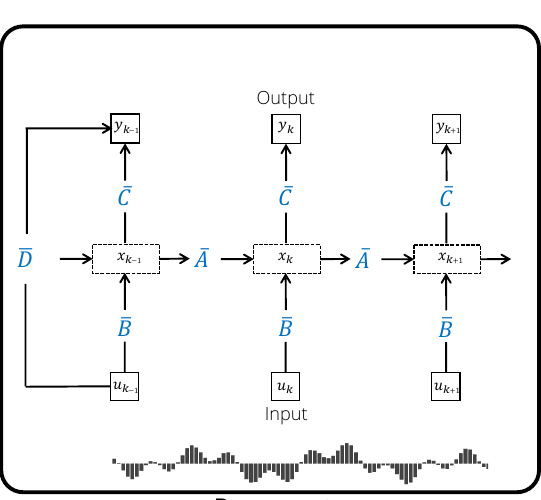
\includegraphics[height=3.48cm]{lssl_recurrent_principle_crop.png}\par
      \vspace{0.04cm}
      {\fontsize{8.0}{9.2}\selectfont
        \(\displaystyle h_t=\bar A h_{t-1}+\bar Bx_t,
        \qquad y_t=Ch_t+Dx_t\)\par}
      \vspace{0.08cm}
      \begin{itemize}\tightitems
        \item \smallnote{\(h_t\in\mathbb{R}^{N}\) có kích thước cố định, tóm tắt toàn bộ lịch sử \(x_{1:t}\); các token cũ không được giữ riêng.}
        \item \smallnote{\(\bar A,\bar B,C,D\) không đổi theo \(t\): hệ tuyến tính bất biến theo thời gian; tính toán tăng theo \(O(L)\).}
      \end{itemize}
    \end{column}
    \begin{column}{0.48\textwidth}
      \heading{Self-attention: lưu KV của toàn bộ token}
      \vspace{0.05cm}
      \centering
      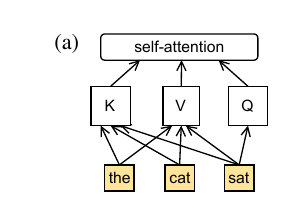
\includegraphics[width=5.05cm]{self_attention_tokens_crop.png}\par
      \vspace{0.04cm}
      {\fontsize{7.6}{8.8}\selectfont
        \(\displaystyle \mathrm{KVCache}_t=
        [(K_1,V_1),\ldots,(K_t,V_t)]\)\par
        \vspace{0.06cm}
        \(\displaystyle y_t=
        \operatorname{softmax}\!\left(\frac{Q_tK_{1:t}^{\mathsf T}}{\sqrt{d_k}}\right)V_{1:t}\)\par}
      \vspace{0.08cm}
      \begin{itemize}\tightitems
        \item \smallnote{Query hiện tại \(Q_t\) so khớp với mọi \(K_i\), sau đó tổng hợp thông tin từ toàn bộ \(V_i\).}
        \item \smallnote{KV cache tăng theo độ dài ngữ cảnh; khi huấn luyện, \(QK^{\mathsf T}\in\mathbb{R}^{L\times L}\) tạo chi phí \(O(L^2)\).}
      \end{itemize}
    \end{column}
  \end{columns}
\end{frame}

% Slide 4
\begin{frame}{1. Bối cảnh nghiên cứu: Hạn chế và mục tiêu}
  \vspace{0.05cm}
  \begin{columns}[T,onlytextwidth]
    \begin{column}{0.322\textwidth}
      \begin{tcolorbox}[equalpanel]
        \heading{Transformer}
        \vspace{0.12cm}
        \begin{itemize}\tightitems
          \item Self-attention cho phép tương tác trực tiếp giữa mọi cặp token.
          \item Dense attention có thời gian và bộ nhớ huấn luyện tăng theo \(O(L^2)\).
          \item Suy luận tự hồi quy cần KV cache tăng theo độ dài ngữ cảnh.
        \end{itemize}
      \end{tcolorbox}
    \end{column}
    \begin{column}{0.322\textwidth}
      \begin{tcolorbox}[equalpanel]
        \heading{Mô hình dưới bậc hai}
        \vspace{0.12cm}
        \begin{itemize}\tightitems
          \item RNN, linear attention, convolution và structured SSM giảm chi phí theo \(L\).
          \item Các mô hình trước Mamba chưa đạt chất lượng attention trên ngôn ngữ.
          \item Nguyên nhân chính được bài báo xác định: thiếu suy luận phụ thuộc nội dung.
        \end{itemize}
      \end{tcolorbox}
    \end{column}
    \begin{column}{0.322\textwidth}
      \begin{tcolorbox}[equalpanel]
        \heading{Mục tiêu của Mamba}
        \vspace{0.12cm}
        \begin{itemize}\tightitems
          \item Bổ sung khả năng chọn thông tin cần ghi nhớ hoặc loại bỏ theo input.
          \item Duy trì thời gian tính toán tuyến tính theo chiều dài chuỗi.
          \item Xây dựng backbone chung cho dữ liệu rời rạc và liên tục.
        \end{itemize}
      \end{tcolorbox}
    \end{column}
  \end{columns}
  \vspace{0.20cm}
  \begin{tcolorbox}[keypanel]
    \centering\bfseries Bài toán đặt ra: nén ngữ cảnh dài vào trạng thái hữu hạn, đồng thời duy trì khả năng chọn lọc thông tin theo nội dung.
  \end{tcolorbox}
\end{frame}

% Slide 4
\begin{frame}{2. Tổng quan Selective State Space Model}
  \vspace{-0.04cm}
  \centering
  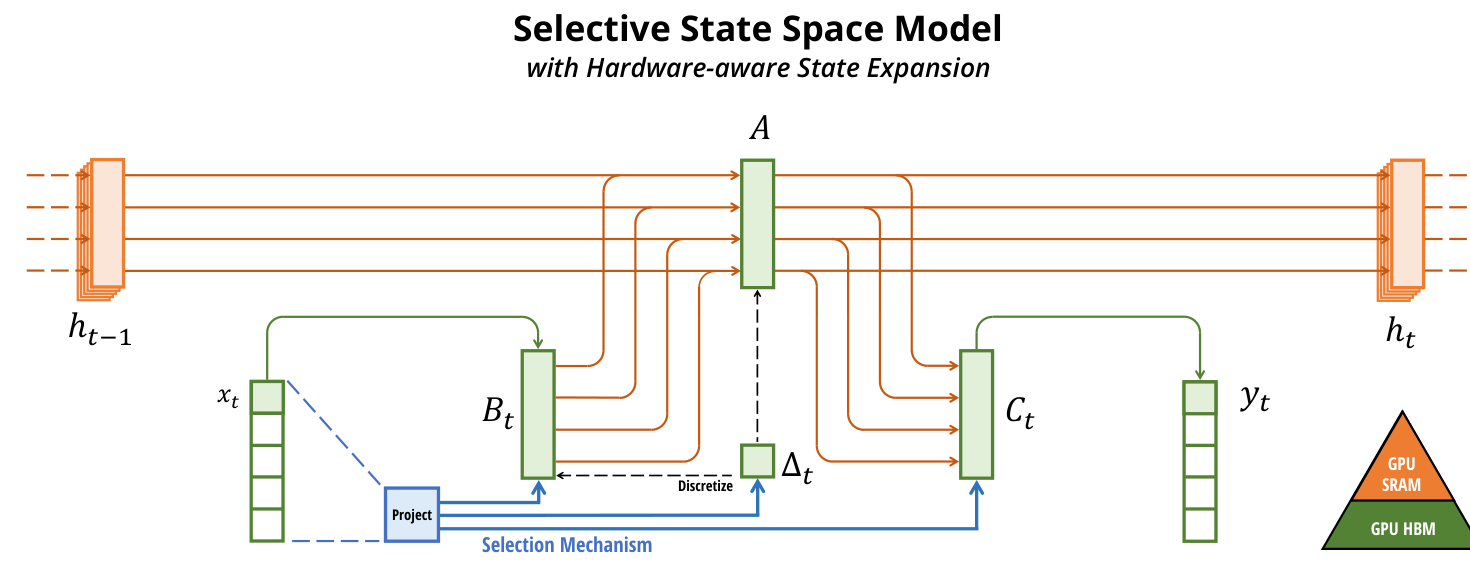
\includegraphics[width=0.78\linewidth]{figure_1_overview.png}
  \vspace{0.02cm}
  \begin{columns}[T,onlytextwidth]
    \begin{column}{0.49\textwidth}
      \begin{tcolorbox}[titlepanel,title=Selection trong mô hình trạng thái]
        \smallnote{Input \(x_t\) sinh \(B_t,C_t,\Delta_t\). State \(h_t\) nén lịch sử; \(B_t\) điều khiển ghi, \(C_t\) điều khiển đọc, \(\Delta_tA\) điều khiển chuyển trạng thái.}
      \end{tcolorbox}
    \end{column}
    \begin{column}{0.49\textwidth}
      \begin{tcolorbox}[titlepanel,title=Thiết kế phù hợp phần cứng]
        \smallnote{State expansion được tạo và xử lý trong SRAM; HBM chỉ lưu input, tham số cần thiết và output. Mục tiêu là giảm memory I/O của recurrence.}
      \end{tcolorbox}
    \end{column}
  \end{columns}
\end{frame}

% Slide 5
\begin{frame}{3. Nền tảng SSM: Từ hệ liên tục đến chuỗi rời rạc}
  \vspace{0.02cm}
  \begin{columns}[T,onlytextwidth]
    \begin{column}{0.48\textwidth}
      \begin{tcolorbox}[titlepanel,title=Vì sao cần rời rạc hóa?]
        \smallnote{SSM xuất phát từ hệ động lực liên tục theo thời gian. Trong mạng nơ-ron, dữ liệu được đưa vào theo từng token hoặc frame, nên state phải được cập nhật tại các bước rời rạc.}
        \vspace{0.05cm}
        \centering
        \(\displaystyle \mathbf h'(t)=\mathbf A\mathbf h(t)+\mathbf Bx(t),
        \quad y(t)=\mathbf C\mathbf h(t)\)\par
        \vspace{0.06cm}
        {\color{PTITRed}\bfseries\(\Downarrow\quad\) lấy mẫu với bước \(\Delta\)\par}
        \vspace{0.06cm}
        \(\displaystyle \mathbf h_t=\overline{\mathbf A}\mathbf h_{t-1}
        +\overline{\mathbf B}x_t,
        \quad y_t=\mathbf C\mathbf h_t\)\par
        \vspace{0.08cm}
        \tinytext{Với zero-order hold: \(\overline{\mathbf A}=\exp(\Delta\mathbf A)\); \(\overline{\mathbf B}\) tích lũy tác động của input trong khoảng thời gian \(\Delta\).}
      \end{tcolorbox}
    \end{column}
    \begin{column}{0.50\textwidth}
      \begin{tcolorbox}[titlepanel,title=Hai cách tính sau khi rời rạc hóa]
        \smallnote{Khi \(\Delta,\mathbf A,\mathbf B,\mathbf C\) cố định theo timestep, cùng một hệ rời rạc có hai cách triển khai tương đương:}
        \vspace{0.14cm}
        \renewcommand{\arraystretch}{1.28}
        \begin{tabularx}{\linewidth}{@{}L{1.80cm}Y C{1.55cm}@{}}
          \toprule
          \textbf{Dạng} & \textbf{Vai trò} & \textbf{Chi phí}\\
          \midrule
          Recurrence & Suy luận tuần tự, state cố định. & \(O(1)\)/bước\\
          Convolution & Huấn luyện song song bằng kernel toàn cục. & \(O(L\log L)\)\\
          \bottomrule
        \end{tabularx}
      \end{tcolorbox}
    \end{column}
  \end{columns}
  \vspace{0.18cm}
  \begin{tcolorbox}[keypanel]
    \textbf{Ý nghĩa của rời rạc hóa:} chuyển động lực học liên tục thành recurrence chạy một lần tại mỗi token/frame. \(\Delta\) xác định lượng thời gian liên tục tương ứng với một bước chuỗi; giả thiết LTI giữ quy tắc chuyển state không đổi giữa các bước.
  \end{tcolorbox}
\end{frame}

% Slide 6
\begin{frame}{4. Selection như một cơ chế nén ngữ cảnh}
  \vspace{-0.08cm}
  \centering
  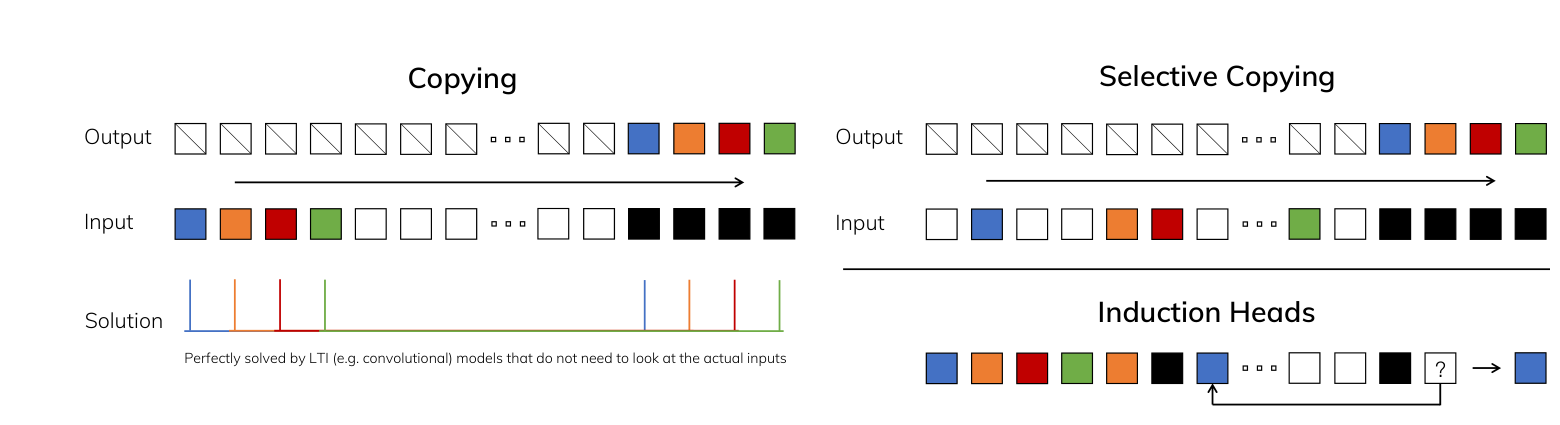
\includegraphics[width=0.97\linewidth]{figure_2_synthetic_tasks_wide.png}\par
  \vspace{0.08cm}
  \begin{columns}[T,onlytextwidth]
    \begin{column}{0.49\textwidth}
      \begin{tcolorbox}[titlepanel,title=Selective Copying,height=1.72cm,valign=top]
        \smallnote{Vị trí token cần nhớ thay đổi giữa các token nhiễu. State phải chọn thông tin để ghi theo nội dung; LTI/convolution cố định không thể chỉ dựa vào khoảng cách.}
      \end{tcolorbox}
    \end{column}
    \begin{column}{0.49\textwidth}
      \begin{tcolorbox}[titlepanel,title=Induction Heads,height=1.72cm,valign=top]
        \smallnote{Khi cặp \([A,B]\) đã xuất hiện, gặp lại \(A\) phải truy hồi \(B\). Bài toán kiểm tra associative recall và khả năng truy xuất thông tin trong ngữ cảnh dài.}
      \end{tcolorbox}
    \end{column}
  \end{columns}
\end{frame}

% Slide 7
\begin{frame}{5. Thuật toán S4 và Selective SSM S6}
  \vspace{0.00cm}
  \begin{columns}[T,onlytextwidth]
    \begin{column}{0.49\textwidth}
      \begin{tcolorbox}[titlepanel,title=Algorithm 1: SSM (S4)]
        {\fontsize{7.4}{8.8}\selectfont
        \renewcommand{\arraystretch}{1.20}
        \begin{tabularx}{\linewidth}{@{}L{1.55cm}Y@{}}
          \textbf{Input} & \(x:(B,L,D)\)\\
          \textbf{Parameters} & \(A:(D,N),\ B:(D,N),\ C:(D,N),\ \Delta:(D)\)\\
          \midrule
          \textbf{Discretize} & \(\overline A,\overline B:(D,N)\leftarrow \mathrm{discretize}(\Delta,A,B)\)\\
          \textbf{Transform} & \(y:(B,L,D)\leftarrow \mathrm{SSM}(\overline A,\overline B,C)(x)\)\\
          \textbf{Return} & \(y\)\\
        \end{tabularx}}
      \end{tcolorbox}
      \vspace{0.14cm}
      \begin{tcolorbox}[panel]
        \smallnote{Tham số không có chiều \(L\); lớp là LTI và có thể tính bằng global convolution.}
      \end{tcolorbox}
    \end{column}
    \begin{column}{0.49\textwidth}
      \begin{tcolorbox}[titlepanel,title=Algorithm 2: SSM + Selection (S6)]
        {\fontsize{7.4}{8.8}\selectfont
        \renewcommand{\arraystretch}{1.20}
        \begin{tabularx}{\linewidth}{@{}L{1.55cm}Y@{}}
          \textbf{Input} & \(x:(B,L,D)\)\\
          \textbf{Parameter} & \(A:(D,N)\)\\
          \textbf{Selection} & \(B:(B,L,N)\leftarrow s_B(x)\)\\
          & \(C:(B,L,N)\leftarrow s_C(x)\)\\
          & \(\Delta:(B,L,D)\leftarrow \tau_\Delta(\mathrm{Param}+s_\Delta(x))\)\\
          \midrule
          \textbf{Discretize} & \(\overline A,\overline B:(B,L,D,N)\)\\
          \textbf{Transform} & \(y:(B,L,D)\leftarrow \mathrm{SSM}(\overline A,\overline B,C)(x)\)\\
        \end{tabularx}}
      \end{tcolorbox}
      \vspace{0.14cm}
      \begin{tcolorbox}[panel]
        \smallnote{Tham số có chiều \(L\); lớp trở thành time-varying và phải được tính bằng recurrence/scan.}
      \end{tcolorbox}
    \end{column}
  \end{columns}
\end{frame}

% Slide 8
\begin{frame}{6. Cơ chế vận hành của Selective SSM}
  \vspace{0.00cm}
  \begin{columns}[T,onlytextwidth]
    \begin{column}{0.48\textwidth}
      \begin{tcolorbox}[titlepanel,title=Vai trò của \(\Delta_t\)]
        \smallnote{Với \(N=1\), \(A=-1\), \(B=1\), selective SSM rút gọn thành recurrence có gate:}
        \[g_t=\sigma(\mathrm{Linear}(x_t))\]
        \[h_t=(1-g_t)h_{t-1}+g_tx_t\]
        \begin{itemize}\tightitems
          \item \(\Delta_t\) nhỏ: duy trì state, giảm ảnh hưởng của input hiện tại.
          \item \(\Delta_t\) lớn: tập trung vào input hiện tại, làm mờ state trước đó.
        \end{itemize}
      \end{tcolorbox}
    \end{column}
    \begin{column}{0.50\textwidth}
      \begin{tcolorbox}[titlepanel,title={Vai trò của \(B_t\), \(C_t\) và \(A\)}]
        \begin{itemize}\tightitems
          \item \(B_t\) điều khiển cách input \(x_t\) được ghi vào state \(h_t\).
          \item \(C_t\) điều khiển phần thông tin trong state được đọc thành output \(y_t\).
          \item \(A\) không cần selective vì selectivity đã đi vào \(\overline A_t=\exp(\Delta_tA)\).
          \item Kết hợp \(\Delta_t,B_t,C_t\) cho phép context filtering và boundary resetting.
        \end{itemize}
      \end{tcolorbox}
      \vspace{0.14cm}
      \begin{tcolorbox}[keypanel]
        \smallnote{Selection không chỉ là phép nhân gate trong kiến trúc; nó trực tiếp thay đổi động lực học lan truyền state dọc chiều thời gian.}
      \end{tcolorbox}
    \end{column}
  \end{columns}
\end{frame}

% Slide 9
\begin{frame}{7. Thuật toán selective scan tối ưu phần cứng}
  \vspace{0.00cm}
  \begin{columns}[T,onlytextwidth]
    \begin{column}{0.35\textwidth}
      \begin{tcolorbox}[titlepanel,title=Thách thức triển khai]
        \begin{itemize}\tightitems
          \item Selection phá vỡ dạng global convolution của S4.
          \item Recurrence mở rộng state thành tensor \((B,L,D,N)\).
          \item Materialize state trong HBM tạo chi phí memory I/O lớn.
          \item Recurrence cần được song song hóa để khai thác GPU.
        \end{itemize}
      \end{tcolorbox}
      \vspace{0.14cm}
      \begin{tcolorbox}[panel]
        \smallnote{Mục tiêu triển khai: giữ tensor mở rộng trong SRAM và chỉ ghi output \((B,L,D)\) về HBM.}
      \end{tcolorbox}
    \end{column}
    \begin{column}{0.63\textwidth}
      \begin{tcolorbox}[titlepanel,title=Thiết kế của bài báo]
        {\fontsize{7.6}{9.0}\selectfont
        \renewcommand{\arraystretch}{1.22}
        \begin{tabularx}{\linewidth}{@{}L{2.00cm}Y L{1.85cm}@{}}
          \toprule
          \textbf{Kỹ thuật} & \textbf{Cách thực hiện} & \textbf{Tác động}\\
          \midrule
          Kernel fusion & Fuse discretization, scan và projection \(C_t\) trong một GPU kernel; state expansion nằm trong SRAM. & Giảm đọc/ghi HBM.\\
          Parallel scan & Dùng toán tử kết hợp để tổ chức recurrence theo cây song song. & Công việc \(O(L)\), khai thác GPU.\\
          Recomputation & Tính lại state trong backward thay vì lưu toàn bộ activation. & Giảm bộ nhớ huấn luyện.\\
          \bottomrule
        \end{tabularx}}
      \end{tcolorbox}
    \end{column}
  \end{columns}
\end{frame}

% Slide 10
\begin{frame}{8. Kiến trúc Mamba}
  \vspace{-0.02cm}
  \centering
  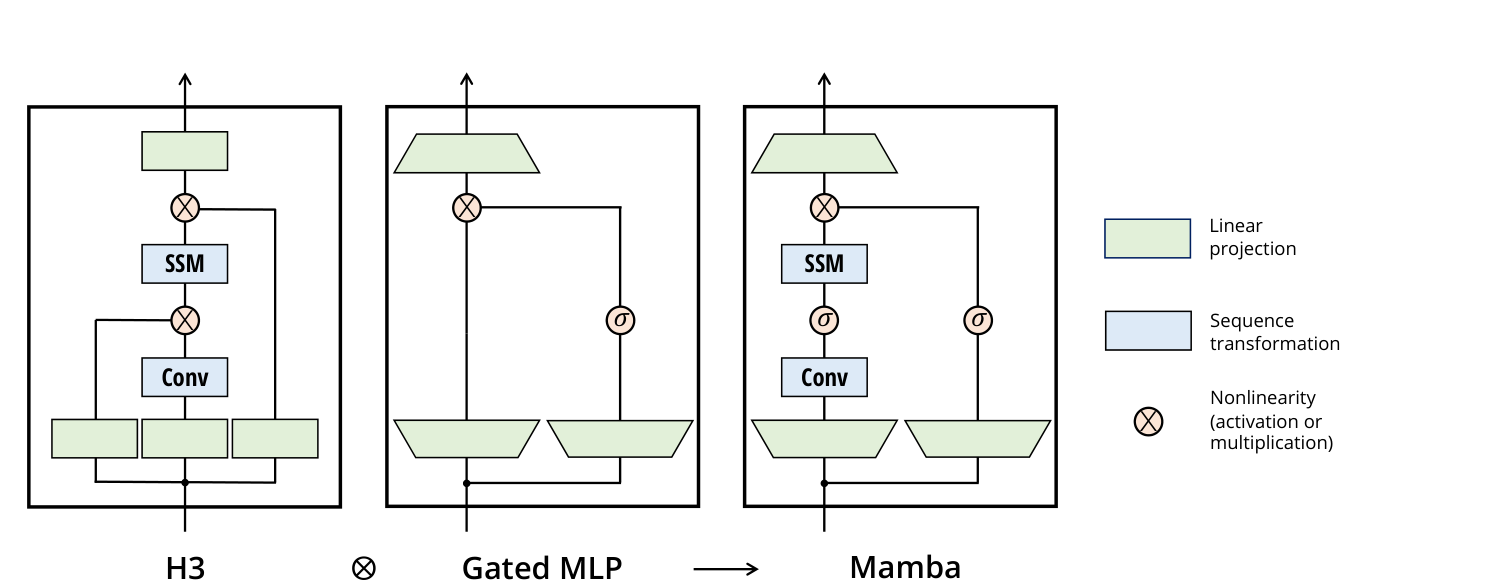
\includegraphics[width=0.78\linewidth]{figure_3_architecture.png}
  \vspace{0.02cm}
  \begin{columns}[T,onlytextwidth]
    \begin{column}{0.32\textwidth}
      \begin{tcolorbox}[panel]
        \textbf{Nhánh biến đổi chuỗi}\par
        \smallnote{Linear projection \(\rightarrow\) short Conv1D \(\rightarrow\) SiLU \(\rightarrow\) selective SSM.}
      \end{tcolorbox}
    \end{column}
    \begin{column}{0.32\textwidth}
      \begin{tcolorbox}[panel]
        \textbf{Nhánh điều biến}\par
        \smallnote{Linear projection \(\rightarrow\) SiLU; nhân theo phần tử với đầu ra nhánh SSM.}
      \end{tcolorbox}
    \end{column}
    \begin{column}{0.32\textwidth}
      \begin{tcolorbox}[panel]
        \textbf{Block đồng nhất}\par
        \smallnote{Output projection và residual; không cần xen kẽ attention block với MLP block.}
      \end{tcolorbox}
    \end{column}
  \end{columns}
  \vspace{0.00cm}
  \tinytext{Mamba kết hợp H3-style sequence transformation và gated MLP thành một block duy nhất; expansion factor mặc định \(E=2\), state dimension thường dùng \(N=16\).}
\end{frame}

% Slide 11
\begin{frame}{9. Bằng chứng trên các bài toán tổng hợp}
  \vspace{0.00cm}
  \begin{columns}[T,onlytextwidth]
    \begin{column}{0.42\textwidth}
      \begin{tcolorbox}[titlepanel,title=Selective Copying]
        \renewcommand{\arraystretch}{1.18}
        \begin{tabularx}{\linewidth}{@{}Y L{1.15cm}R{0.90cm}@{}}
          \toprule
          \textbf{Architecture} & \textbf{Layer} & \textbf{Acc.}\\
          \midrule
          No gate & S4 & 18.3\\
          H3 & S4 & 57.0\\
          H3 & Hyena & 30.1\\
          H3 & S6 & 99.7\\
          \textbf{Mamba} & \textbf{S6} & \textbf{99.8}\\
          \bottomrule
        \end{tabularx}
      \end{tcolorbox}
      \vspace{0.14cm}
      \begin{tcolorbox}[panel]
        \smallnote{Kết quả tách biệt ảnh hưởng của architectural gating và selection: thay S4 bằng S6 tạo cải thiện quyết định.}
      \end{tcolorbox}
    \end{column}
    \begin{column}{0.56\textwidth}
      \centering
      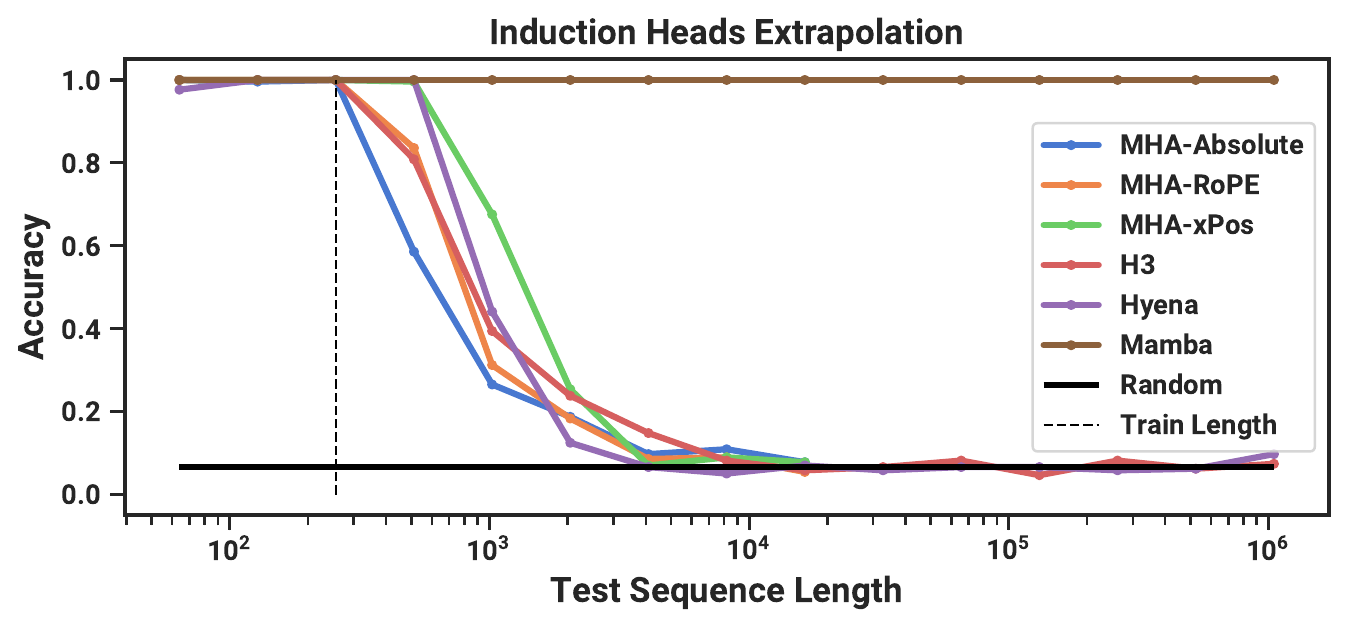
\includegraphics[width=\linewidth]{figure_2_induction_heads.png}
      \vspace{0.04cm}
      \smallnote{Mô hình huấn luyện tại \(L=256\). Mamba duy trì accuracy gần hoàn hảo tới \(L=2^{20}\), trong khi H3, Hyena và các biến thể attention suy giảm hoặc bị giới hạn bộ nhớ.}
    \end{column}
  \end{columns}
\end{frame}

% Slide 12
\begin{frame}{10. So sánh Mamba và các kiến trúc khác}
  \vspace{0.04cm}
  \renewcommand{\arraystretch}{1.38}
  \begin{tabularx}{\linewidth}{@{}L{2.15cm}L{3.15cm}Y L{3.20cm}@{}}
    \toprule
    \textbf{Miền dữ liệu} & \textbf{Thiết lập chính} & \textbf{Kết quả của Mamba} & \textbf{Ý nghĩa kiến trúc}\\
    \midrule
    Language modeling & The Pile; mô hình tới 2.8B tham số & Mamba-2.8B đạt average 63.3 trên 6 benchmark, vượt Pythia-2.8B và RWKV-3B. & Selection khắc phục điểm yếu của LTI SSM trên token rời rạc.\\
    DNA & HG38; context từ \(2^{10}\) tới \(2^{20}\) & Perplexity tiếp tục cải thiện tới khoảng một triệu base pair; vượt HyenaDNA theo context. & State chọn lọc khai thác ngữ cảnh rất dài thay vì tích lũy nhiễu.\\
    Audio & YouTubeMix và SC09 waveform & Pretraining cải thiện tới gần một triệu sample; FID SC09 đạt 0.67 ở mô hình 24.3M. & Mamba vẫn hiệu quả trên modality liên tục, nhưng tồn tại đánh đổi LTI--selective.\\
    \bottomrule
  \end{tabularx}
  \vspace{0.22cm}
  \begin{tcolorbox}[keypanel]
    \centering Đối với video, các kết quả này chỉ chứng minh năng lực backbone chuỗi tổng quát; bài báo chưa đánh giá trực tiếp action recognition hoặc triển khai edge.
  \end{tcolorbox}
\end{frame}

% Slide 13
\begin{frame}{11. Hiệu quả tính toán và khả năng triển khai}
  \vspace{-0.02cm}
  \centering
  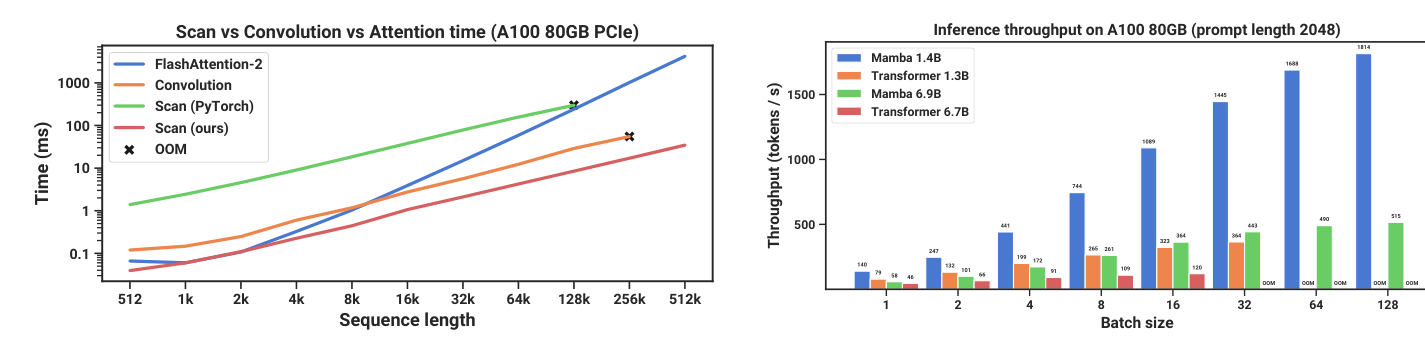
\includegraphics[width=0.86\linewidth]{figure_8_efficiency_benchmarks.png}
  \vspace{0.05cm}
  \begin{columns}[T,onlytextwidth]
    \begin{column}{0.32\textwidth}
      \begin{tcolorbox}[panel]
        \centering\bfseries Phép toán selective scan\par
        \smallnote{Nhanh hơn scan PyTorch 20--40 lần; vượt FlashAttention-2 trong phép toán lõi từ khoảng 2K token.}
      \end{tcolorbox}
    \end{column}
    \begin{column}{0.32\textwidth}
      \begin{tcolorbox}[panel]
        \centering\bfseries Suy luận tự hồi quy\par
        \smallnote{Throughput cao hơn Transformer cùng kích thước khoảng 4--5 lần trong benchmark A100.}
      \end{tcolorbox}
    \end{column}
    \begin{column}{0.32\textwidth}
      \begin{tcolorbox}[panel]
        \centering\bfseries Bộ nhớ\par
        \smallnote{Không cần KV cache tăng theo \(L\); memory huấn luyện tương đương Transformer dùng FlashAttention-2.}
      \end{tcolorbox}
    \end{column}
  \end{columns}
  \vspace{0.10cm}
  \tinytext{Các số liệu trên đo trên NVIDIA A100 80GB; không thể suy ra trực tiếp latency trên Jetson, NPU hoặc CPU edge.}
\end{frame}

% Slide 15
\begin{frame}{12. Mức độ phù hợp với bài toán Action Recognition}
  \vfill
  \begin{columns}[T,onlytextwidth]
    \begin{column}{0.49\textwidth}
      \begin{tcolorbox}[titlepanel,title=Giới hạn từ bài báo]
        \begin{itemize}\tightitems
          \item Quy mô language model đánh giá tối đa khoảng 3B tham số.
          \item Hệ sinh thái fine-tuning, quantization và adaptation chưa được khảo sát hệ thống.
          \item Selection có thể làm suy yếu inductive bias liên tục mà LTI SSM vốn khai thác tốt.
          \item Benchmark hiệu quả thực hiện trên GPU A100, không phải thiết bị biên.
        \end{itemize}
      \end{tcolorbox}
    \end{column}
    \begin{column}{0.49\textwidth}
      \begin{tcolorbox}[titlepanel,title=Khoảng trống đối với video]
        \begin{itemize}\tightitems
          \item Mamba chỉ mô hình hóa chuỗi feature; thông tin không gian vẫn cần CNN hoặc ViT backbone.
          \item Nén toàn bộ lịch sử vào state hữu hạn có thể mất chi tiết chuyển động ngắn hạn.
          \item Offline recognition có thể cần ngữ cảnh hai chiều; selective scan gốc mang tính causal.
          \item Kernel tối ưu của Mamba có thể không sẵn có trên NPU, TensorRT hoặc CPU edge.
        \end{itemize}
      \end{tcolorbox}
    \end{column}
  \end{columns}
  \vfill
\end{frame}

% Slide 17
\begin{frame}{13. Kết luận}
  \vspace{0.16cm}
  \begin{columns}[T,onlytextwidth]
    \begin{column}{0.32\textwidth}
      \begin{tcolorbox}[equalpanel,height=5.15cm]
        \heading{Đóng góp mô hình hóa}
        \vspace{0.12cm}
        {\fontsize{7.10}{8.20}\selectfont
        \textcolor{PTITRed}{\bfseries Tham số chọn lọc}\par
        \(B_t,C_t,\Delta_t=s(x_t)\); dynamics nền \(A\) vẫn cố định.\par
        \vspace{0.12cm}
        \textcolor{PTITRed}{\bfseries Cơ chế ghi--giữ--đọc}\par
        \(\Delta_t\) điều khiển mức cập nhật; \(B_t\) ghi input vào state; \(C_t\) đọc state để tạo output.\par
        \vspace{0.12cm}
        \textcolor{PTITRed}{\bfseries Kết quả}\par
        State trở thành bộ nhớ phụ thuộc nội dung; selection giải quyết bài toán sao chép chọn lọc và khái quát induction sang chuỗi dài hơn huấn luyện.\par}
      \end{tcolorbox}
    \end{column}
    \begin{column}{0.32\textwidth}
      \begin{tcolorbox}[equalpanel,height=5.15cm]
        \heading{Đóng góp thuật toán}
        \vspace{0.12cm}
        {\fontsize{7.10}{8.20}\selectfont
        \textcolor{PTITRed}{\bfseries Fused selective scan}\par
        Hợp nhất rời rạc hóa, scan và phép chiếu; giữ state expansion trong SRAM để giảm trao đổi HBM.\par
        \vspace{0.12cm}
        \textcolor{PTITRed}{\bfseries Song song và bộ nhớ}\par
        Parallel scan giữ công việc tuyến tính theo \(L\); recomputation giảm activation memory; suy luận dùng state cố định, không cần KV cache tăng theo ngữ cảnh.\par}
      \end{tcolorbox}
    \end{column}
    \begin{column}{0.32\textwidth}
      \begin{tcolorbox}[equalpanel,height=5.15cm]
        \heading{Kiến trúc và đánh giá}
        \vspace{0.12cm}
        {\fontsize{7.10}{8.20}\selectfont
        \textcolor{PTITRed}{\bfseries Mamba block}\par
        Short Conv1D, SiLU, selective SSM và multiplicative gate được hợp nhất trong residual block đồng nhất, không sử dụng attention.\par
        \vspace{0.12cm}
        \textcolor{PTITRed}{\bfseries Kết quả benchmark}\par
        Kết quả mạnh trên language, DNA, audio và tác vụ tổng hợp cần chọn lọc ngữ cảnh dài.\par
        \vspace{0.12cm}
        \textcolor{PTITRed}{\bfseries Phạm vi}\par
        Mô hình dưới khoảng 3B tham số, đo hiệu quả trên A100; chưa đánh giá trực tiếp video, Action Recognition hoặc thiết bị biên.\par}
      \end{tcolorbox}
    \end{column}
  \end{columns}
\end{frame}

% Slide 17
\begin{frame}{14. Tiến độ triển khai phát hiện người cần phục vụ cho robot}
  \vspace{-0.03cm}
  \begin{columns}[T,onlytextwidth]
    \begin{column}{0.56\textwidth}
      \begin{tcolorbox}[titlepanel,title=So sánh mô hình nano pose]
        {\fontsize{7.2}{8.4}\selectfont
        \renewcommand{\arraystretch}{1.25}
        \begin{tabularx}{\linewidth}{@{}Y C{1.50cm} C{1.55cm} C{1.18cm}@{}}
          \toprule
          \textbf{Chỉ số} & \textbf{YOLOv8n-pose} & \textbf{YOLO26n-pose} & \textbf{Thay đổi}\\
          \midrule
          COCO pose mAP$_{50:95}$ & 50.4 & \textbf{57.2} & +6.8 điểm\\
          Tham số & 3.3 M & \textbf{2.9 M} & $-12\%$\\
          FLOPs tại 640 px & 9.2 B & \textbf{7.5 B} & $-18\%$\\
          \bottomrule
        \end{tabularx}}
      \end{tcolorbox}
      \vspace{0.12cm}
      \begin{tcolorbox}[panel]
        \smallnote{YOLO26n-pose thay YOLOv8n-pose vì đạt độ chính xác cao hơn với ít tham số và FLOPs hơn.}
      \end{tcolorbox}
    \end{column}
    \begin{column}{0.42\textwidth}
      \centering
      
\includegraphics[height=3.05cm]{skeleton.png}\par
      \vspace{0.04cm}
      \smallnote{Sơ đồ keypoint dùng để minh họa skeleton và kiểm tra điều kiện vẫy tay của người mục tiêu.}
    \end{column}
  \end{columns}
  \vspace{-0.18cm}
  \begin{tcolorbox}[titlepanel,title=Luồng triển khai phát hiện người]
    {\fontsize{6.5}{7.5}\selectfont
    \setlength{\tabcolsep}{1.2pt}
    \begin{tabularx}{\linewidth}{@{}C{1.65cm} c C{2.25cm} c C{1.65cm} c C{1.35cm} c C{1.20cm} c Y@{}}
      \textbf{YOLO26n-pose FP32} & $\rightarrow$ & \textbf{Export ONNX FP16, ONNX Runtime} & $\rightarrow$ & \textbf{TensorRT \texttt{.engine}} & $\rightarrow$ & \textbf{Jetson run} & $\rightarrow$ & \textbf{Skeleton} & $\rightarrow$ & \textbf{Check wave condition}
    \end{tabularx}}
  \end{tcolorbox}
\end{frame}

% Slide 18
\begin{frame}[t]{15. Tiến độ triển khai phát hiện người cần phục vụ cho robot}
  \vspace{0.02cm}
  \begin{columns}[T,onlytextwidth]
    \begin{column}{0.42\textwidth}
      \begin{tcolorbox}[titlepanel,title=Hạn chế hiện tại,height=4.55cm,valign=top]
        \begin{itemize}\tightitems
          \item Khoảng cách phát hiện tối đa trong thử nghiệm hiện tại khoảng \textbf{5 m}.
          \item Hệ thống mới chỉ xử lý ổn định \textbf{một người} trong khung hình.
          \item Khi xuất hiện thêm người, FPS giảm mạnh, gây giật/lag và làm hệ thống có nguy cơ quá tải.
        \end{itemize}
      \end{tcolorbox}
    \end{column}
    \begin{column}{0.56\textwidth}
      \begin{tcolorbox}[titlepanel,title=Hướng triển khai đề xuất,height=4.55cm,valign=top]
        \begin{itemize}\tightitems
          \item Dùng mô hình \textbf{person detection} nhẹ để lấy bounding box.
          \item Crop từng ROI người; phân tích skeleton bằng mô hình nhẹ như \textbf{MediaPipe Pose}.
          \item Thêm \textbf{object tracking} để duy trì ID và vị trí người giữa các frame.
          \item Áp dụng \textbf{frame skipping}: cập nhật detection/pose theo chu kỳ, dùng tracking ở các frame trung gian.
        \end{itemize}
      \end{tcolorbox}
    \end{column}
  \end{columns}
  \vspace{0.16cm}
  \begin{tcolorbox}[panel]
    {\fontsize{7.1}{8.3}\selectfont\centering
      \textbf{Person detector} $\rightarrow$ \textbf{Bounding box} $\rightarrow$ \textbf{Crop ROI} $\rightarrow$ \textbf{MediaPipe Pose} $\rightarrow$ \textbf{Tracking + frame skipping} $\rightarrow$ \textbf{Wave condition}\par}
  \end{tcolorbox}
\end{frame}

\end{document}
